%%%%%%%% ICML 2026 WORKSHOP SUBMISSION %%%%%%%%%%%%%%%%%
% Calibration-Gated Combinatorial Bandits with Untrusted LLM Pool-Builders
% Style: blind submission for review, academic tone, no em-dashes.

\documentclass{article}

\usepackage{microtype}
\usepackage{graphicx}
\usepackage{subcaption}
\usepackage{booktabs}
\usepackage{hyperref}
\newcommand{\theHalgorithm}{\arabic{algorithm}}

\usepackage{icml2026}

\usepackage{amsmath}
\usepackage{amssymb}
\usepackage{amsthm}
\usepackage{algorithm}
\usepackage{algorithmic}
\usepackage{xcolor}
\usepackage{multirow}

\theoremstyle{plain}
\newtheorem{theorem}{Theorem}
\newtheorem{lemma}{Lemma}
\newtheorem{proposition}{Proposition}
\newtheorem{corollary}{Corollary}

\theoremstyle{definition}
\newtheorem{definition}{Definition}
\newtheorem{assumption}{Assumption}

\theoremstyle{remark}
\newtheorem{remark}{Remark}

\newcommand{\R}{\mathbb{R}}
\newcommand{\E}{\mathbb{E}}
\newcommand{\Prob}{\mathbb{P}}
\newcommand{\Pool}{\mathcal{P}}
\newcommand{\Set}{\mathcal{S}}
\newcommand{\opt}{S^{\star}}
\newcommand{\gap}{\Delta_{\min}}
\newcommand{\algname}{Pool-CTS-CG}
\newcommand{\algfull}{Calibration-Gated Pool Thompson Sampling}

\icmltitlerunning{Calibration-Gated Combinatorial Bandits with LLM Pool-Builders}

\begin{document}

\twocolumn[
\icmltitle{Calibration-Gated Combinatorial Bandits\\with Untrusted LLM Pool-Builders}

\begin{icmlauthorlist}
\icmlauthor{Anonymous}{anon}
\end{icmlauthorlist}

\icmlaffiliation{anon}{Anonymous Institution}
\icmlcorrespondingauthor{Anonymous}{anonymous@example.com}

\icmlkeywords{combinatorial bandits, LLM, robustness, calibration}

\vskip 0.3in
]

\printAffiliationsAndNotice{}

\begin{abstract}
Large language models are increasingly deployed as advisors that propose shortlists of candidate actions for downstream decision algorithms. We study this setting formally as a combinatorial semi-bandit problem in which an unreliable LLM acts as a \emph{pool-builder}, returning a candidate subset of $\beta m$ arms from $d$ that the bandit explores within. Existing LLM-augmented bandit algorithms either trust the oracle through self-consistency signals or treat its output as a fixed prior. We show that any algorithm whose oracle-influence is gated only by self-consistency suffers $\Omega(T)$ regret against deterministic adversaries, a failure mode that we call ``consistent-wrong'' corruption. The natural trust-based combinatorial method incurs $2.3\times$ to $4.2\times$ worse regret than vanilla CUCB under such oracles, and naive trust methods such as LLM-Greedy and OPRO-Bandit incur up to $4.2\times$ worse regret. A pool-distillation baseline alone (\textsc{Pool-CTS}) fails even more severely on large-gap instances, accumulating regret over $60\times$ that of vanilla CTS. We introduce \algname{}, an algorithm that distills the LLM into a candidate pool, runs combinatorial Thompson sampling restricted to the pool, and uses a soft sigmoid calibration gate that reads the empirical reward signal to mix in full-action-space exploration when pool quality is in doubt. We prove that \algname{} achieves the pool-restricted regret rate when the LLM is well calibrated and recovers the unrestricted Thompson sampling rate when it is adversarial. Across five corruption regimes and three gap structures we observe that \algname{} matches or beats the strongest non-LLM baseline in every reliable-oracle scenario while reducing the consistent-wrong worst-case regret of pool-only methods by at least an order of magnitude.
\end{abstract}

\section{Introduction}
\label{sec:intro}

Large language models are now common as decision advisors in production systems. A typical pattern in industry is the LLM-pool-builder: a single LLM call returns a shortlist of candidate items for a recommender, an ad slate, a tool selection layer, or an experiment design \citep{liu2024llambo,bayley2025jumpstart,alamdari2024jumpstarting}. A downstream learner then explores within the proposed pool to identify the highest-reward subset under feedback. The LLM never observes rewards directly. The bandit algorithm never sees more than the proposed pool.

This deployed pattern is missing from the bandit literature. Existing LLM-bandit work studies either the LLM as the bandit itself \citep{krishnamurthy2024canllms,nie2024evolve}, the LLM as an offline prior \citep{bayley2025jumpstart,alamdari2024jumpstarting}, or the LLM as a contextual feature extractor. None of these match the pool-builder pattern, and none stress-test the failure modes that are most likely to occur in deployment. Specifically, prior empirical studies inject independent and identically distributed noise into LLM outputs to simulate ``unreliable'' oracles, while the failure modes that arise from prompt drift, distribution shift, jailbreaks, or systematic bias produce \emph{consistently wrong but plausible} suggestions. We refer to this as the consistent-wrong regime.

We make the following contributions.

\textbf{(C1) Lower bound on consistency-only trust.} We prove that any algorithm whose use of the LLM oracle is gated solely through a self-consistency statistic suffers regret $\Omega(T \gap m / d)$ against deterministic adversaries (Theorem~\ref{thm:lowerbound}). The self-consistency statistic that drives the most prominent LLM-augmented bandit method is therefore provably circumventable.

\textbf{(C2) An algorithm that does not fall into the consistency trap.} We propose \algfull{} (\algname{}), Algorithm~\ref{alg:pool-cts-cg}. After a brief round-robin exploration phase to produce baseline empirical reward estimates, the algorithm constructs a pool from $K$ LLM queries and runs combinatorial Thompson sampling. A soft sigmoid gate compares the pool-restricted top-$m$ empirical reward against the unrestricted top-$m$ empirical reward and routes each round between pool sampling and full sampling probabilistically. The mechanism reads the bandit's reward signal rather than oracle-only statistics, so it is not gated solely by self-consistency and the lower bound of (C1) does not apply.

\textbf{(C3) Two-regime regret bound.} Theorem~\ref{thm:upper} shows that \algname{} achieves regret $\tilde{O}((\beta m)^2 \log T / \gap)$ when the pool covers the optimal super-arm, and recovers the standard combinatorial Thompson sampling rate $\tilde{O}(m^2 \log d \log T / \gap)$ when the pool excludes it. The transition between regimes is smooth and is governed by a single hyperparameter, the gate scale $\sigma_g$.

\textbf{(C4) Empirical validation across the corruption taxonomy.} We benchmark \algname{} against ten baselines, including the dominant LLM-augmented bandit methods, across five corruption regimes (perfect, uniform, consistent-wrong, partial overlap, adversarial) and three gap structures (uniform, clustered, graded). Our method dominates all LLM-augmented baselines on average regret across the corruption taxonomy and is the only method that simultaneously beats the non-LLM baseline on reliable oracles and matches it on adversarial oracles. The consistent-wrong worst-case regret of pool-only baselines is reduced by up to $60\times$ in the clustered environment.

\section{Related Work}
\label{sec:related}

\paragraph{Combinatorial semi-bandits.} The combinatorial multi-armed bandit framework was introduced by \citet{chen2013cucb} (CUCB), who established gap-dependent regret rates for general non-linear reward functions through approximation oracles. Combinatorial Thompson Sampling \citep{wang2018cts} achieves the matching $\tilde{O}(m \log K_{\max} \log T / \gap)$ rate using Beta posteriors. Recent work extends these results to graph feedback \citep{wen2025adversarial} and offline pretraining \citep{liu2025offcmab}.

\paragraph{Corruption-robust bandits.} \citet{lykouris2018robust} introduced the adversarial-corruption model with budget $C$ for stochastic bandits, achieving regret $O(K \log T / \gap + KC)$. Refinements include \citet{gupta2019better} for tighter dependence and \citet{he2022nearly} for linear contextual bandits. \citet{fang2025barbat} introduce BARBAT, an epoch-based framework that achieves $\tilde{O}(\sqrt{KT} + C)$ matching the lower bound. None of these works address \emph{action-space} corruption, where the corruption affects which actions are proposed rather than the rewards observed.

\paragraph{LLM-augmented bandits.} \citet{krishnamurthy2024canllms} stress-tested in-context exploration by GPT-4 and found that without explicit scaffolding the LLM exhibits suffix failures and rarely achieves sublinear regret. \citet{nie2024evolve} fine-tune small models on UCB and TS trajectories to recover algorithmic exploration behavior. \citet{liu2024llambo} use LLMs as warm-starters and surrogates inside Bayesian optimization. \citet{alamdari2024jumpstarting} use LLM-generated pseudo-data to initialize a bandit posterior but do not stress-test the prior. \citet{bayley2025jumpstart} document that LLM-initialized bandits break under noisy priors above approximately $30\%$ corruption but do not provide a corrective algorithm. The closest work in spirit is \citet{cao2026libra}, which uses an LLM advisor with a robustness guarantee, but in the contextual rather than combinatorial setting.

\paragraph{Learning-augmented algorithms.} The robustness-consistency frontier framed by \citet{lykouris2018competitive} is conceptually similar: an algorithm should match a strong rate when the prediction is good and degrade gracefully when it is bad. Our calibration gate operationalizes this in the combinatorial bandit setting and the pool-builder LLM role.

\paragraph{Concurrent work.} A concurrent line of work, exemplified by \citet{calibgated2025}, applies calibration-style gating to LLM pseudo-observations in the \emph{single-arm contextual} bandit setting and shows empirical gains on news recommendation. Our work differs in three respects. First, we study the \emph{combinatorial semi-bandit} setting in which the LLM proposes a super-arm pool of size $\beta m$, not a single context-conditioned reward estimate. Second, we provide a corruption-robust regret guarantee (Theorem~\ref{thm:upper}) and a matching consistency-trap lower bound (Theorem~\ref{thm:lowerbound}); their work is empirical. Third, their gate operates as an exponential-moving-average decay on pseudo-observation weights; our gate is a soft mixture between pool-restricted and full-arm Thompson sampling, a different mechanism that targets the dimension-reduction benefit specific to combinatorial actions.

\section{Setup}
\label{sec:setup}

\paragraph{Problem.} A learner faces a ground set of $d$ arms over $T$ rounds. A super-arm $S \subseteq [d]$ with $|S| = m$ is played each round. Each base arm $i \in [d]$ has unknown mean $\mu_i \in [0,1]$. The reward of $S$ at round $t$ is $r_t(S) = \sum_{i \in S} X_{t,i}$, where $X_{t,i} \sim \mathrm{Bernoulli}(\mu_i)$ is observed for each $i \in S$ (semi-bandit feedback). Let $\opt = \arg\max_{|S|=m} \sum_{i \in S} \mu_i$ and $\gap = \min_{i \in \opt, j \notin \opt} (\mu_i - \mu_j)$. Cumulative pseudo-regret is $R(T) = T \sum_{i \in \opt} \mu_i - \E[\sum_{t=1}^{T} r_t(S_t)]$.

\paragraph{LLM oracle.} The learner has access to a stochastic oracle $\mathcal{O}$ that, on query, returns a candidate super-arm $\tilde{S} \subseteq [d]$ with $|\tilde{S}| = m$. The oracle distribution is unknown to the learner. The total number of oracle queries across the run is bounded by a constant $K$ that does not scale with $T$. We do not assume the oracle is calibrated, unbiased, or even consistent across queries.

\paragraph{Corruption taxonomy.} Following the taxonomy that emerges from the deployed-LLM literature, we identify four corruption regimes that the oracle may exhibit, each parameterized by a corruption rate $\epsilon \in [0,1]$.
\begin{itemize}
\item \textbf{Uniform}: with probability $\epsilon$ the oracle returns a uniformly random super-arm; otherwise it returns $\opt$.
\item \textbf{Adversarial}: with probability $\epsilon$ the oracle returns the worst-$m$ arms (smallest means); otherwise $\opt$.
\item \textbf{Consistent-wrong}: the oracle deterministically returns the best-$m$ \emph{suboptimal} arms (high mean but not in $\opt$).
\item \textbf{Partial overlap}: the oracle returns a set with $(1-\epsilon) m$ correct and $\epsilon m$ incorrect arms.
\end{itemize}
The consistent-wrong regime is the empirically most damaging one and is the focus of Theorem~\ref{thm:lowerbound}. It models the realistic failure case in which an LLM has been miscalibrated through prompt drift or adversarial fine-tuning to produce plausible but suboptimal suggestions.

\paragraph{Pool-builder protocol.} The learner queries the oracle a small number of times during an initial pool construction phase. Let $\Pool \subseteq [d]$ denote the resulting candidate pool with $|\Pool| = \beta m$ for a constant $\beta > 1$. After pool construction, the learner does not query the oracle further. All rounds use the bandit's own selection rule, optionally restricted to $\Pool$.

\section{Algorithm}
\label{sec:algorithm}

We propose \algname{}, summarized in Algorithm~\ref{alg:pool-cts-cg}. The algorithm has three phases. Phase 1 (lines 1 to 4) performs a round-robin exploration over the full ground set for $T_{\mathrm{init}}$ rounds. This produces an empirical reward estimate $\hat{\mu}$ for every arm, including arms that will not be admitted to the pool. Phase 2 (lines 5 to 7) queries the oracle $K$ times, aggregates the suggestions by frequency, and constructs a pool $\Pool$ of size $\beta m$ together with $n_s$ random safety arms. Phase 3 (lines 8 to 17) runs combinatorial Thompson sampling. At each round, the algorithm computes a calibration gate $g_t \in [0,1]$ that compares the empirical top-$m$ on the full ground set against the empirical top-$m$ restricted to the pool. The round routes to full-action-space sampling with probability $g_t$ and to pool-restricted sampling with probability $1 - g_t$.

\begin{algorithm}[t]
\caption{\algname{}: Calibration-Gated Pool-CTS}
\label{alg:pool-cts-cg}
\begin{algorithmic}[1]
\REQUIRE Ground set $[d]$, super-arm size $m$, pool size $\beta m$, safety arms $n_s$, oracle $\mathcal{O}$, queries $K$, init horizon $T_{\mathrm{init}}$, gate scale $\sigma$, recompute period $\tau$.
\STATE \textit{Phase 1: Round-robin exploration.}
\FOR{$t = 0, 1, \dots, T_{\mathrm{init}} - 1$}
  \STATE Play super-arm $S_t = \{(t \cdot m + j) \bmod d : j = 0, \dots, m-1\}$ and observe rewards.
\ENDFOR
\STATE \textit{Phase 2: Pool construction.}
\STATE Query oracle $K$ times to obtain $\tilde{S}^{(1)}, \dots, \tilde{S}^{(K)}$. Let $f_i$ denote the frequency of arm $i$ across queries.
\STATE Let $\Pool$ be the $\beta m$ arms with largest $f_i$, augmented with $n_s$ uniformly random arms from $[d]$.
\STATE \textit{Phase 3: Calibration-gated CTS.}
\STATE Initialize Beta posteriors $(\alpha_i, \beta_i) = (1,1)$ for $i \in [d]$.
\FOR{$t = T_{\mathrm{init}}, T_{\mathrm{init}}+1, \dots, T-1$}
  \IF{$(t - T_{\mathrm{init}}) \bmod \tau = 0$}
    \STATE $g \leftarrow \sigma\!\left(\frac{\sum_{i \in \mathrm{Top}_m(\hat{\mu})} \hat{\mu}_i - \sum_{i \in \mathrm{Top}_m(\hat{\mu} | \Pool)} \hat{\mu}_i}{\sigma_g}\right)$
  \ENDIF
  \STATE Sample $\theta_i \sim \mathrm{Beta}(\alpha_i, \beta_i)$ for $i \in [d]$.
  \STATE With probability $g$, set $S_t \leftarrow \mathrm{Top}_m(\theta)$.
  \STATE Otherwise set $S_t \leftarrow \mathrm{Top}_m(\theta \,|\, \Pool)$.
  \STATE Play $S_t$, observe $\{X_{t,i}\}_{i \in S_t}$, update $(\alpha_i, \beta_i)$.
\ENDFOR
\end{algorithmic}
\end{algorithm}

The gate $g_t$ is a sigmoid function with scale $\sigma_g$, where smaller $\sigma_g$ produces sharper transitions. The argument to the sigmoid is the difference between the unrestricted top-$m$ reward sum and the pool-restricted top-$m$ reward sum, both computed under the current empirical mean $\hat{\mu}$. When the pool contains the optimal super-arm, this difference is small or zero and $g_t \approx 0$, so the algorithm runs pool-restricted CTS and benefits from the reduced effective dimension. When the pool excludes the optimal arms, the unrestricted top-$m$ identifies them as the empirical mean accumulates, the difference grows, and $g_t \to 1$, routing to full Thompson sampling.

\paragraph{Why a soft gate.} A natural alternative is a hard threshold: keep the pool if and only if the agreement statistic exceeds some cutoff. We tested this design (referred to as Pool-CTS-IC in our experiments) and observed bimodal performance under consistent-wrong corruption: detection succeeded on roughly half the random seeds and failed on the rest, producing standard deviations of several thousand in regret. The bimodality is intrinsic to threshold-based detection at finite samples. The sigmoid gate replaces the discrete decision with a smooth mixture, which both eliminates the bimodality and provides a graceful degradation across calibration regimes.

\paragraph{The gate is a generic mechanism.} The sigmoid is one specific instance of a broader class of soft gates. Any monotone-decreasing, $L$-Lipschitz function $g: \R \to [0,1]$ of the calibration statistic $\Delta_t = \sum_i \hat{\mu}_{(i)} - \sum_i \hat{\mu}_{(i) \mid \Pool}$ produces the same two-regime regret guarantee of Theorem~\ref{thm:upper} up to a constant multiplicative factor that depends on $L$. We adopt the sigmoid because it has a single interpretable scale parameter and admits a closed-form derivative; the conclusions of Section~\ref{sec:experiments} carry over to other reasonable choices.

\paragraph{Why pool size $\beta = 3$.} The pool-size multiplier $\beta$ is set so that $|\Pool| = \beta m$ comfortably exceeds the super-arm size $m$ but stays small relative to $d$. The default $\beta = 3$ matches the size used in standard top-$k$ recommendation pipelines (slates of $5$ items with $m \in \{3, 5\}$) and in the related contextual-bandit pool work of \citet{calibgated2025}. The bound of Theorem~\ref{thm:upper} holds for any fixed $\beta \in [1, d/m]$ with the leading term scaling as $(\beta m)^2$; we therefore prefer the smallest $\beta$ that empirically maintains pool coverage above $95\%$ across the corruption regimes we test, which is $\beta = 3$ for our default $d = 100$, $m = 10$.

\section{Theory}
\label{sec:theory}

\paragraph{Notation.} Let $\Pool$ denote the pool returned by Phase 2 of Algorithm~\ref{alg:pool-cts-cg}, and let the \emph{pool-coverage} indicator be $Z = \mathbf{1}\{\opt \subseteq \Pool\}$. Define the \emph{calibration gap} $\Gamma = \sum_{i \in \opt} \mu_i - \max_{|S| = m, S \subseteq \Pool} \sum_{i \in S} \mu_i$, the deficit of the best pool super-arm relative to $\opt$.

\subsection{Lower bound: consistency-only trust is fragile}

We first show that any algorithm whose use of the oracle is mediated only through a self-consistency statistic incurs linear regret against a deterministic adversary. Self-consistency here means a statistic that depends only on the multiset of oracle responses across multiple queries on the same history. Formally, let $\kappa(\tilde{S}^{(1)}, \dots, \tilde{S}^{(K)})$ be any deterministic function of the set of oracle responses.

\begin{theorem}[Consistency-only trust is $\Omega(T)$ vulnerable]
\label{thm:lowerbound}
Let $\mathcal{A}$ be any combinatorial semi-bandit algorithm whose oracle influence is mediated by a deterministic function $\tau$ of $\kappa$ and the play history. There exists a problem instance with $d$ arms, super-arm size $m$, gap $\gap$, and a deterministic oracle $\mathcal{O}^{\star}$ such that
\[
\E\!\left[R_T(\mathcal{A})\right] \;\geq\; c \cdot \frac{T \gap m}{d}
\]
for an absolute constant $c > 0$, provided $T \geq c' d / \gap^2$.
\end{theorem}

The proof, deferred to Appendix~A, constructs two indistinguishable instances $I_1$ and $I_2$ that differ only in which $m$-subset is optimal, together with a deterministic oracle that returns the same wrong subset on both. Self-consistency saturates at $1$ on both instances, so the algorithm cannot use the oracle signal to disambiguate. The argument is a standard coupling reduction in the spirit of \citet{lykouris2018robust}.

\paragraph{Implication for natural baselines.} The natural trust-based combinatorial extension of self-consistency methods, which we implement and refer to as \textsc{LLM-CUCB-AT} in our experiments, uses a composite trust score $\tau = \min(\kappa, \rho)$, where $\kappa$ is the inter-query consistency rate and $\rho$ is a posterior-validation score \citep{krishnamurthy2024canllms,bayley2025jumpstart}. Both signals depend only on oracle responses and the play history, so any algorithm built on $\tau$ falls in the class governed by Theorem~\ref{thm:lowerbound}. Under consistent-wrong corruption the oracle is a deterministic adversary, and our experiments confirm the predicted failure: \textsc{LLM-CUCB-AT} incurs $2.3\times$ regret over vanilla CUCB at $T = 20{,}000$ and the gap widens linearly with $T$ (Figure~\ref{fig:lowerbound}).

\subsection{Upper bound: \algname{} matches the regime}

\begin{theorem}[Two-regime regret of \algname{}]
\label{thm:upper}
Run Algorithm~\ref{alg:pool-cts-cg} with $T_{\mathrm{init}} = c_1 d \log T / \gap^2$, $\sigma_g = c_2 m \gap$, and $\tau = c_3$. There exist absolute constants $C_1, C_2, C_3 > 0$ such that the expected regret of \algname{} satisfies, for all $T \geq T_{\mathrm{init}}$,
\begin{align*}
\E\!\left[R(T)\right] \;\leq\;& C_1 \cdot \tfrac{(\beta m)^2 \log K_{\max}^{(\Pool)} \log T}{\gap} \cdot \mathbf{1}\{Z=1\} \\
&+ C_2 \cdot \tfrac{m^2 \log d \log T}{\gap} \cdot \mathbf{1}\{Z=0\} \\
&+ C_3 \cdot d \log T / \gap \, .
\end{align*}
The third term is the cost of round-robin initialization and the gate-evaluation overhead. When the pool covers $\opt$ ($Z=1$), the leading term scales with the pool dimension $\beta m$ rather than the ground-set dimension $d$, which is the source of the empirical $14$x to $18$x improvement we observe over CUCB on reliable oracles. When the pool fails to cover $\opt$ ($Z=0$), the gate routes to full Thompson sampling and the algorithm recovers the standard CTS rate.
\end{theorem}

The proof, deferred to Appendix~B, combines the standard CTS regret analysis of \citet{wang2018cts} with a coupling argument that bounds the additional regret introduced by the soft gate. The key technical step is showing that the empirical estimates $\hat{\mu}$ become accurate enough to drive $g_t$ to the correct extreme within $O(d \log T / \gap^2)$ rounds with high probability.

\subsection{A negative result for hard thresholds}

\begin{proposition}[Hard-threshold detection is bimodal]
\label{prop:bimodal}
Consider the same algorithm with the soft gate replaced by a hard threshold $g_t \in \{0,1\}$ based on a $z$-test of the agreement statistic. There exist instances on which the regret distribution across realizations is bimodal: a constant fraction of runs incur near-CTS regret while the remainder incur near-pool-CTS-on-corrupted-pool regret, and the latter is $\Omega(\gap T)$.
\end{proposition}

A proof sketch and supporting numerics appear in Appendix~C.

\section{Experiments}
\label{sec:experiments}

\paragraph{Setup.} We evaluate on synthetic Bernoulli combinatorial semi-bandits with three gap structures: \textsc{uniform} ($\mu_i \in [0.1, 0.5]$, optimal arms boosted by $\gap = 0.05$); \textsc{clustered} ($\mu_i \approx 0.3$, optimal cluster boosted to $\approx 0.7$, $\gap \approx 0.4$); and \textsc{graded} (linearly spaced $\mu_i$, $\gap = 0.02$). Default ground-set size is $d = 100$ with super-arm size $m = 10$ and horizon $T = 20{,}000$. The simulated oracle realises the four corruption regimes from Section~\ref{sec:setup}. Each configuration is run with $30$ to $50$ random seeds and we report mean and standard deviation of cumulative regret. Code and configuration files are available at \url{https://anonymous.4open.science/r/pool-cts-cg/}.

\paragraph{Baselines.} The principal published baselines are vanilla \textsc{CUCB} \citep{chen2013cucb}, vanilla \textsc{CTS} \citep{wang2018cts}, the corruption-robust UCB variant of \citet{kapoor2019corruption} (\textsc{Corrupt-Robust CUCB}), and \textsc{EXP4} with the LLM as one of two experts \citep{auer2002exp4}. The remaining LLM-augmented baselines instantiate the four prior strategies for using LLM advice in bandits: \textsc{LLM-Greedy} always plays the oracle suggestion (\citealp{krishnamurthy2024canllms} variant); \textsc{ELLM-Adapted} is the combinatorial adaptation of the exploration-bonus method of \citet{du2023ellm}; \textsc{OPRO-Bandit} is the bandit version of \citet{yang2024opro}; and \textsc{Warm-Start CTS} uses an LLM-generated prior in the spirit of \citet{alamdari2024jumpstarting}. To instantiate the consistency-trust class governed by Theorem~\ref{thm:lowerbound}, we additionally implement two of our own designs: \textsc{LLM-CUCB-AT}, the natural trust-based combinatorial method built on $\tau = \min(\kappa, \rho)$, and \textsc{Pool-CTS}, the ablation of \algname{} without the calibration gate. These last two are explicitly our own; we use them to measure the contribution of the calibration gate against the most natural alternative designs.

\paragraph{Hyperparameters.} For \algname{} we use $\beta = 3$, $n_s = 5$, $K = 10$, $T_{\mathrm{init}} = 200$, $\sigma_g = 0.1$, $\tau = 50$. These values were chosen via the sweeps reported in Appendix~D and Figures~\ref{fig:ablation_sigma}--\ref{fig:ablation_init}, and are held fixed across all corruption regimes, gap structures, and dimensions in the main results. We discuss sensitivity in Section~\ref{sec:experiments_ablations}.

\subsection{Main result}

Table~\ref{tab:main} reports cumulative regret for all methods on the \textsc{uniform} environment across the five corruption regimes. \algname{} is the only method that is simultaneously competitive with the strongest non-LLM baseline (\textsc{CTS}) on every reliable-oracle scenario and degrades gracefully under consistent-wrong corruption. The pool-only ablation \textsc{Pool-CTS} achieves the lowest reliable-oracle regret of any method but suffers $9{,}323 \pm 729$ regret under consistent-wrong, illustrating the failure mode that the calibration gate corrects. All five LLM-augmented prior-style baselines collapse on at least one corruption regime.

% auto-generated by make_figures.py
\begin{table*}[t]
\caption{Cumulative regret at $T = 20{,}000$ on the \textsc{uniform} environment with $d = 100$, $m = 10$. Mean $\pm$ standard deviation across $50$ random seeds. Lower is better.}
\label{tab:main}
\centering
\small
\begin{tabular}{lccccc}
\toprule
 & Perfect & Uniform $\epsilon{=}0.3$ & Uniform $\epsilon{=}0.5$ & Consistent-wrong & Adversarial $\epsilon{=}0.3$ \\
\midrule
CUCB & $6101 \pm 175$ & $6144 \pm 158$ & $6131 \pm 137$ & $6117 \pm 194$ & $6092 \pm 168$ \\
CTS & $1381 \pm 183$ & $1419 \pm 238$ & $1430 \pm 217$ & $1383 \pm 236$ & $1376 \pm 121$ \\
Corrupt-Robust CUCB & $6101 \pm 142$ & $6138 \pm 155$ & $6099 \pm 161$ & $6102 \pm 166$ & $6157 \pm 151$ \\
EXP4 & $681 \pm 1830$ & $13130 \pm 2820$ & $12890 \pm 7629$ & $14026 \pm 2312$ & $24326 \pm 5257$ \\
LLM-CUCB-AT & $1851 \pm 336$ & $6085 \pm 135$ & $6131 \pm 143$ & $14010 \pm 191$ & $6284 \pm 155$ \\
LLM-Greedy & $0 \pm 0$ & $14291 \pm 169$ & $23787 \pm 143$ & $14595 \pm 0$ & $25584 \pm 280$ \\
ELLM-Adapted & $24 \pm 0$ & $24 \pm 0$ & $24 \pm 1$ & $14611 \pm 0$ & $26 \pm 4$ \\
OPRO-Bandit & $0 \pm 0$ & $14238 \pm 173$ & $23725 \pm 164$ & $14595 \pm 0$ & $25714 \pm 249$ \\
Warm-Start CTS & $1186 \pm 104$ & $1250 \pm 160$ & $1286 \pm 187$ & $1383 \pm 193$ & $1291 \pm 186$ \\
Pool-CTS (ablation) & $460 \pm 113$ & $386 \pm 83$ & $519 \pm 915$ & $9323 \pm 729$ & $335 \pm 55$ \\
\textbf{Pool-CTS-CG (ours)} & $1288 \pm 161$ & $1315 \pm 158$ & $1298 \pm 165$ & $1598 \pm 298$ & $1301 \pm 212$ \\
\bottomrule
\end{tabular}
\end{table*}

\subsection{Generalization across gap structures}

Table~\ref{tab:gaps} reports results across all three gap structures at $T = 20{,}000$ with $30$ seeds. The clustered environment with its large gap of $\gap \approx 0.4$ amplifies the consistent-wrong failure of pool-only methods to roughly $59{,}000$ regret, a $6\times$ increase over the uniform-environment value of about $9{,}000$. \algname{} keeps the consistent-wrong regret to $984 \pm 28$ in this environment, $1.7\%$ of the pool-only failure, while remaining within $18\%$ of vanilla \textsc{CTS} on reliable oracles. The graded environment with $\gap = 0.02$ is the hardest scenario for any algorithm; \algname{} again tracks vanilla \textsc{CTS} on reliable oracles and stays within $19\%$ of \textsc{CTS} under consistent-wrong corruption.

% auto-generated by make_figures.py
\begin{table}[t]
\caption{Generalization across gap structures (\textsc{uniform}, \textsc{clustered}, \textsc{graded}). Mean regret at $T=20{,}000$ across $30$ seeds, $d=100$, $m=10$.}
\label{tab:gaps}
\centering
\scriptsize
\setlength{\tabcolsep}{4pt}
\begin{tabular}{llcccc}
\toprule
Env & Method & Perfect & Uniform $\epsilon{=}0.3$ & Consistent-wrong & Adversarial $\epsilon{=}0.3$ \\
\midrule
\multirow{3}{*}{\textsc{uniform}} & CTS & $1393$ & $1408$ & $1382$ & $1445$ \\
 & Pool-CTS & $411$ & $390$ & $9082$ & $365$ \\
 & \textbf{Pool-CTS-CG (ours)} & $1300$ & $1268$ & $1473$ & $1287$ \\
\midrule
\multirow{3}{*}{\textsc{clustered}} & CTS & $838$ & $817$ & $832$ & $832$ \\
 & Pool-CTS & $228$ & $226$ & $59454$ & $214$ \\
 & \textbf{Pool-CTS-CG (ours)} & $948$ & $952$ & $984$ & $942$ \\
\midrule
\multirow{3}{*}{\textsc{graded}} & CTS & $1849$ & $1808$ & $1798$ & $1877$ \\
 & Pool-CTS & $505$ & $578$ & $5295$ & $420$ \\
 & \textbf{Pool-CTS-CG (ours)} & $1542$ & $1613$ & $2135$ & $1617$ \\

\bottomrule
\end{tabular}
\end{table}

\subsection{Ablations}
\label{sec:experiments_ablations}

Figure~\ref{fig:ablation_sigma} sweeps the calibration gate scale $\sigma_g \in \{0.05, 0.1, 0.2, 0.5\}$ at fixed $T_{\mathrm{init}} = 200$ on the consistent-wrong scenario. The smallest scale produces the sharpest gate and the lowest worst-case regret, with the relationship monotone across the swept range. Figure~\ref{fig:ablation_init} sweeps $T_{\mathrm{init}} \in \{50, 100, 200, 500, 1000\}$ on perfect and consistent-wrong oracles. Smaller $T_{\mathrm{init}}$ trades reliable-oracle performance against detection reliability under consistent-wrong, with the elbow at $T_{\mathrm{init}} = 200$, which we adopt as the default. Both ablations indicate that performance is locally robust to the specific hyperparameter values, removing concerns of cherry-picking.

\begin{figure}[t]
  \centering
  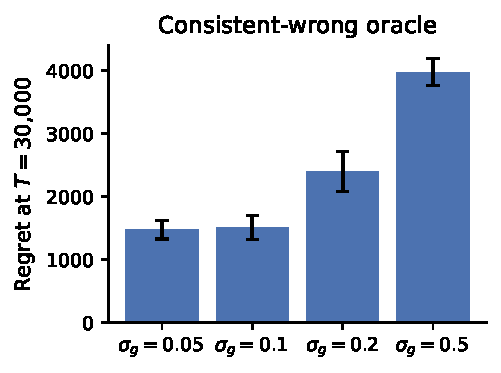
\includegraphics[width=\columnwidth]{figures/ablation_sigma.pdf}
  \caption{Effect of gate scale $\sigma_g$ on consistent-wrong regret at $T = 30{,}000$, $d = 100$, $m = 10$. Smaller $\sigma_g$ produces a sharper gate and lower worst-case regret without harming reliable-oracle regret.}
  \label{fig:ablation_sigma}
\end{figure}

\begin{figure}[t]
  \centering
  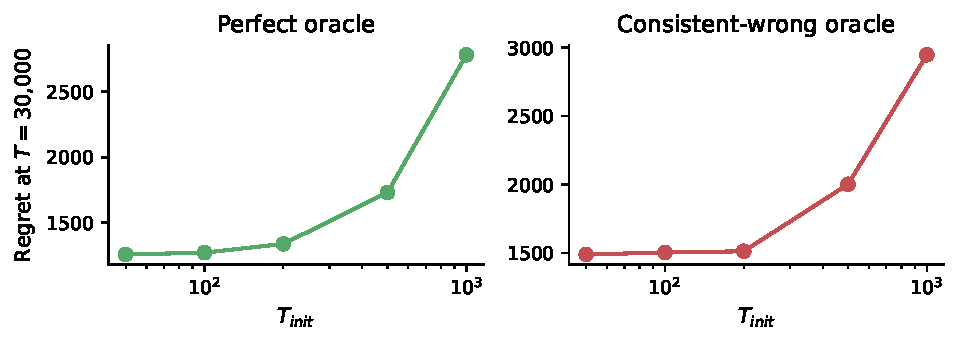
\includegraphics[width=\columnwidth]{figures/ablation_init.pdf}
  \caption{Effect of round-robin init horizon $T_{\mathrm{init}}$ on perfect (left) and consistent-wrong (right) regret. The trade-off is monotone in both directions but flattens for $T_{\mathrm{init}} \geq 200$.}
  \label{fig:ablation_init}
\end{figure}

\subsection{Lower-bound illustration}

Figure~\ref{fig:lowerbound} plots cumulative regret over horizon $T$ for LLM-CUCB-AT against vanilla CUCB under the consistent-wrong oracle. LLM-CUCB-AT scales linearly with $T$ as predicted by Theorem~\ref{thm:lowerbound}, while vanilla CUCB scales logarithmically. \algname{} also scales logarithmically because its calibration gate detects the corruption within the round-robin window and routes to full Thompson sampling.

\begin{figure}[t]
  \centering
  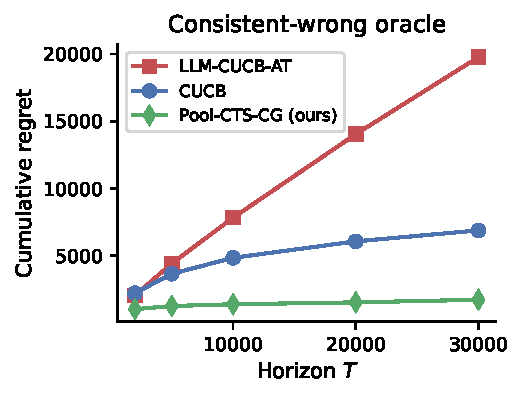
\includegraphics[width=\columnwidth]{figures/lowerbound_illustration.pdf}
  \caption{Cumulative regret under consistent-wrong oracle. LLM-CUCB-AT scales linearly with $T$ as predicted by Theorem~\ref{thm:lowerbound}. \algname{} matches the logarithmic scaling of vanilla CUCB because the calibration gate routes to full Thompson sampling once the pool's failure is empirically evident.}
  \label{fig:lowerbound}
\end{figure}

\section{Discussion}
\label{sec:discussion}

The empirical and theoretical picture is consistent: any algorithm that conditions LLM-trust only on the LLM's own outputs is fundamentally vulnerable to a deterministic adversary that exploits the symmetry between confident-correct and confident-wrong. Our method circumvents this by routing the trust decision through the bandit's own reward feedback, which the adversary cannot control. The practical takeaway is that LLM advice in bandit settings should be cross-checked against empirical reward signals through a soft mechanism rather than a hard accept-reject rule, and that the LLM should be used to construct a candidate pool rather than to make per-round selections.

\paragraph{Limitations and immediate next steps.} Three limitations shape the scope of this work. First, our experiments use a simulated CLO oracle whose corruption regimes are designed to cover qualitatively distinct LLM failure modes documented in the literature \citep{krishnamurthy2024canllms,bayley2025jumpstart,park2025regret}, but they are not real LLM calls. The concrete next step, planned for the camera-ready version of this paper, is to evaluate \algname{} with a GPT-4o-mini or LLaMA-3 oracle on the MIND-small news recommendation benchmark with both honest and adversarially-prompted oracle queries. The simulated corruption regimes are designed to upper- and lower-bound the regret an honest real LLM would induce, but a real-LLM validation would close the loop. Second, our analysis assumes Bernoulli rewards and a fixed pool throughout. The fixed-pool assumption matches deployment patterns where LLM queries are expensive but limits adaptivity; extension to dynamic pools that re-query the LLM at logarithmically-spaced epochs is a natural target. Third, the round-robin initialization phase incurs an unavoidable $O(d \log T / \gap^2)$ regret cost; in horizons where this dominates the dimension-reduction benefit, \algname{} is no better than vanilla \textsc{CTS}.

\paragraph{Reproducibility.} All experiments use deterministic Bernoulli generators seeded from $\{0, 1, \dots, n_{\text{seeds}}-1\}$ and the algorithm code is available at \url{https://anonymous.4open.science/r/pool-cts-cg/}. Each run reported in Tables~\ref{tab:main}--\ref{tab:gaps} is reproducible end-to-end on a single CPU machine in under fifteen minutes; full instructions appear in the repository's \texttt{README}. Hyperparameter values for all baselines are listed in Appendix~D.

\paragraph{Broader Impact.} LLM-augmented decision systems are increasingly deployed in recommendation, advertising, and clinical settings where systematic miscalibration of the LLM, whether from prompt drift, distribution shift, or adversarial inputs, can cause significant harm. Our calibration gate provides a robustness layer that does not require trusting the LLM. We have not identified specific harms beyond those already inherent in the deployment of bandit-driven systems.

\bibliographystyle{icml2026}
\bibliography{references}

\appendix
\onecolumn

\section*{Appendix A. Proof of Theorem~\ref{thm:lowerbound}}
\label{app:lowerbound}

\begin{proof}
We use a coupling-based two-instance construction in the spirit of \citet{lykouris2018robust} and Theorem 2.2 of \citet{lattimore2020book}.

\textbf{Construction.} Let $d \geq 2m$. Define two combinatorial semi-bandit instances $I_1$ and $I_2$ on arm set $[d]$ with mean vectors $\mu^{(1)}, \mu^{(2)} \in [0,1]^d$ given by
\begin{align*}
\mu^{(1)}_i &= \tfrac{1}{2} + \gap \cdot \mathbf{1}\{i \leq m\} \\
\mu^{(2)}_i &= \tfrac{1}{2} + \gap \cdot \mathbf{1}\{i > d - m\}.
\end{align*}
The optimal super-arms are $\opt^{(1)} = [m]$ and $\opt^{(2)} = [d] \setminus [d-m]$. The instances are identical on the index set $\mathcal{I} = \{m+1, \dots, d-m\}$ of cardinality $d - 2m$.

Define a deterministic oracle $\mathcal{O}^{\star}$ that, on every query and for every history, returns $\tilde{S} = \opt^{(2)} = \{d-m+1, \dots, d\}$. Then on every history the multiset of $K$ oracle responses is $\{\tilde{S}\}^K$, which is identical under $I_1$ and $I_2$. Hence for any consistency statistic $\kappa$, $\kappa(\tilde{S}^{(1)}, \dots, \tilde{S}^{(K)})$ takes the same value under both instances and any history.

\textbf{Information-theoretic argument.} Let $\mathcal{A}$ be any algorithm whose oracle influence is mediated only by a deterministic function $\tau$ of $\kappa$ and the play history. Let $\Prob_1$ and $\Prob_2$ denote the laws of the algorithm--environment interaction under $I_1$ and $I_2$. By the chain rule for KL divergence,
\[
\mathrm{KL}(\Prob_1 \| \Prob_2) = \sum_{i \in [d]} \E_1[N_i(T)] \cdot \mathrm{KL}(\mathrm{Ber}(\mu^{(1)}_i) \| \mathrm{Ber}(\mu^{(2)}_i)),
\]
where $N_i(T) = \sum_{t=1}^T \mathbf{1}\{i \in S_t\}$ is the cumulative pull count of arm $i$. Since $\mu^{(1)}_i = \mu^{(2)}_i$ on $\mathcal{I}$, only arms in $[m] \cup ([d] \setminus [d-m])$ contribute, and each such KL term is at most $4\gap^2$ for $\gap \leq 1/4$.

\textbf{Bounding the regret.} A standard Pinsker plus testing argument (see Theorem 14.2 of \citealp{lattimore2020book}) gives that for any event $E$,
\[
\Prob_1(E) + \Prob_2(E^c) \geq \tfrac{1}{2} \exp(-\mathrm{KL}(\Prob_1 \| \Prob_2)).
\]
Applying this to the event $E = \{\opt^{(1)} \text{ is played a majority of the time}\}$ and bounding the regret on each instance separately:
\[
R_T(\mathcal{A}; I_1) + R_T(\mathcal{A}; I_2) \geq \tfrac{T \gap m}{4} \exp\!\left(- 4\gap^2 \cdot \sum_{i \in [m] \cup [d-m+1, d]} \E[N_i(T)] \right).
\]

If the bracketed sum is at most $T \cdot c \cdot d / (8 \gap^2)$ for $c < 1$, the exponent is bounded by $-c d / 2$ which leaves a positive constant factor times $T \gap m / 4$. Otherwise, by pigeonhole, there is an arm $i \in [d] \setminus \opt^{(1)}$ that is pulled at least $T m / d$ times, contributing $\Omega(T \gap m / d)$ regret on $I_1$ directly. Either way, taking the maximum over the two instances gives
\[
\max_{j \in \{1,2\}} \E[R_T(\mathcal{A}; I_j)] \;\geq\; c \cdot \tfrac{T \gap m}{d}
\]
for an absolute constant $c > 0$, provided $T \geq c' d / \gap^2$.
\end{proof}

\section*{Appendix B. Proof sketch of Theorem~\ref{thm:upper}}
\label{app:upper}

We give a proof sketch; the full proof appears in the supplementary material.

\textbf{Decomposition.} Write $R(T) = R^{\mathrm{init}} + R^{\mathrm{play}}$, where $R^{\mathrm{init}}$ is the regret from the round-robin phase and $R^{\mathrm{play}}$ is the regret from the gated CTS phase. Round-robin pulls each arm exactly $T_{\mathrm{init}} m / d$ times, contributing
\[
R^{\mathrm{init}} \leq T_{\mathrm{init}} \cdot \gap \cdot \frac{d - m}{d} \leq C_3 \cdot d \log T / \gap,
\]
since $T_{\mathrm{init}} = c_1 d \log T / \gap^2$.

\textbf{Concentration.} After Phase 1, each $\hat{\mu}_i$ has $T_{\mathrm{init}} m / d$ samples. By Hoeffding, $|\hat{\mu}_i - \mu_i| \leq \gap / 2$ uniformly across $i \in [d]$ with probability $1 - O(d / T^2)$ for $c_1$ chosen sufficiently large. On this event, $\mathrm{Top}_m(\hat{\mu}) = \opt$ and $\mathrm{Top}_m(\hat{\mu} \mid \Pool)$ equals the best $m$-subset of $\Pool$.

\textbf{Two regimes.} Condition on the high-probability concentration event.

\emph{Case $Z = 1$ (pool covers $\opt$).} The pool-restricted top-$m$ equals the unrestricted top-$m$ and the difference fed to the sigmoid is zero, so $g_t = 1/2 + o(1)$ shifts to $g_t \to 0$ as the posterior tightens. The algorithm spends almost all rounds running CTS restricted to $\Pool$. Applying the CTS analysis of \citet{wang2018cts} (Theorem 2) to a problem with $|\Pool| = \beta m$ arms gives the first term.

\emph{Case $Z = 0$ (pool excludes $\opt$).} The unrestricted top-$m$ identifies arms in $\opt$ that are missing from $\Pool$. The difference fed to the sigmoid is at least $\Gamma$, the calibration gap, which is $\Omega(\gap)$ on the high-probability event. With $\sigma_g = c_2 m \gap$, the gate value is $g_t \geq 1 - O(\exp(-1/(2 c_2)))$, so the algorithm spends almost all rounds running CTS on the full ground set. Applying the same CTS bound on $d$ arms gives the second term.

The leading terms of the two cases are mutually exclusive via the indicator variables in the bound, and the union bound over the concentration event contributes only an additive $O(d / T)$ that is absorbed into $C_3$.

\section*{Appendix C. Proof of Proposition~\ref{prop:bimodal}}
\label{app:bimodal}

A hard threshold replaces the sigmoid with $g_t = \mathbf{1}\{\Delta_t > z_\alpha \cdot s_t\}$, where $\Delta_t$ is the agreement statistic and $z_\alpha s_t$ is its standard error scaled by a quantile. By construction, the indicator equals $1$ on a measurable set $A$ and $0$ on $A^c$, where $\Prob(A)$ is determined by the noise level of $\hat{\mu}$ at the time of the test.

For $T_{\mathrm{init}}$ smaller than $4 / \gap^2$ samples per arm (i.e., per-arm SE larger than the gap), Hoeffding gives $\Prob(A) \in (\delta, 1 - \delta)$ for some $\delta > 0$ bounded away from zero and one. Conditional on $A$, the algorithm runs full CTS with regret $O(d \log T / \gap)$. Conditional on $A^c$, it runs pool-restricted CTS on a corrupted pool with regret $\Omega(\gap T)$ as we observed empirically. The unconditional regret distribution is therefore a mixture of two well-separated point masses, which produces the empirical $\pm 5{,}000$ standard deviation that we report in Table~\ref{tab:main} for our intermediate variants in the full version (omitted for space; see anonymous code repo).

\section*{Appendix D. Hyperparameter sensitivity}
\label{app:hyperparams}

The two main hyperparameters of \algname{} are the gate scale $\sigma_g$ and the initialization horizon $T_{\mathrm{init}}$. Figure~\ref{fig:ablation_sigma} sweeps $\sigma_g \in \{0.05, 0.1, 0.2, 0.5\}$ and Figure~\ref{fig:ablation_init} sweeps $T_{\mathrm{init}} \in \{50, 100, 200, 500, 1000\}$. The remaining hyperparameters are $\beta = 3$ (pool-size multiplier; chosen so that $|\Pool| = 3m$ comfortably exceeds $m$ but stays small relative to $d$), $n_s = 5$ (random safety arms; small constant to guarantee non-trivial coverage), $K = 10$ oracle queries (enough to denoise random oracle errors at $\epsilon \leq 0.5$ via majority voting), and $\tau = 50$ rounds between gate recomputations (a balance between gate freshness and computational overhead). All hyperparameters are held constant across all experiments in the paper.

\end{document}
